\documentclass[11pt]{article}

\usepackage{fancyhdr}
\usepackage{hyperref}
\usepackage{graphicx}
\usepackage{enumerate}
\usepackage[greek,dutch]{babel} 
\usepackage{listings}
\usepackage{color}
\usepackage{framed}
\usepackage{subfig}

\usepackage[applemac]{inputenc}
\usepackage[T1]{fontenc}
\usepackage[section]{placeins}

\pagestyle{fancy}


\definecolor{mygreen}{rgb}{0,0.6,0}
\definecolor{mygray}{rgb}{0.5,0.5,0.5}
\definecolor{mymauve}{rgb}{0.58,0,0.82}

\lstset{ %
  backgroundcolor=\color{white},         % size of fonts used for the code
  breaklines=true,                 % automatic line breaking only at whitespace
  captionpos=b,                    % sets the caption-position to bottom
  commentstyle=\color{mygreen},    % comment style
  escapeinside={\%*}{*)},          % if you want to add LaTeX within your code
  keywordstyle=\color{blue},       % keyword style
  stringstyle=\color{mymauve},     % string literal style
}



\interfootnotelinepenalty=10000


\title{Raport Project Databases Maart}
\author{Mathias Beke, Bruno Van de Velde, Elias Van Langenhove, Alexander Vanhulle, Timo Truyts}

\author{
  Mathias Beke
  \and
  Bruno Van de Velde
  \and
  Elias Van Langenhove
  \and
  Alexander Vanhulle
  \and
  Timo Truyts
}


\date{\today}


\setlength{\parindent}{0cm}

\begin{document}

\lhead{Raport Project Databases: Maart}
\rhead{}



\maketitle


\tableofcontents





\section{Status}




\subsection{Taakverdeling}


\begin{enumerate}
    
        \item ERM Schema: samen opgesteld. Digitalisatie: Mathias\footnote{De verdere digitalisatie en verdere aanpassingen werden door Alexander gedaan.}
        
        \item ERM Model omzetten in SQL tables: Alexander, Timo, Elias\footnote{De verfijning hiervan (wat het meeste tijd in beslag neemt) werd vooral door Timo gedaan.}
        
        \item Parser schrijven: Bruno, Mathias\footnote{Bruno heeft zich vooral toegelegd op de parser, en heeft er dan ook veruit het meeste voor gedaan.}
        
        \item Basis datastructuren: Alexander, Elias
        
        \item \emph{Teams} tabel vullen (Bruno)
        
        \item \emph{Coaches} tabel vullen (Bruno)
        
        \item \emph{Player} tabel moet extra informatie meekrijgen zoals lengte, gewicht, positie, geboortedatum, ... Bruno
        
        \item \emph{Date} attribuut van tabellen in orde brengen (Elias)
        
        \item Feitelijk login script, met sessions, registraties, login pagina, ... (Alexander)
        
        \item Verdere implementatie van \emph{get} queries voor de klassen. (Elias)
    
        \item Pagina's en algemeen ontwerp van de site (Timo en Mathias)
        
        \item \emph{Analyse van de data} Timo
        
        \item \emph{Herstructureren van de klassen} Elias      
        
        \item \emph{Crawler die automatisch nieuwe wedstrijden binnenhaalt, en de scores update van gespeelde wedstrijden.} Bruno

        \item \emph{Informatie includen op pagina's} Mathias   

        \item \emph{RSS feed ophalen} Mathias  
        
        \item \emph{Configuratie scherm gebruiker} Alexander     
        
        \item \emph{Pagina's stylen, nadat ze ge\"implementeerd zijn} Alexander\footnote{Alexander heeft vooral de gebruikers- en wed pagina's van een design voorzien. Het algemeen design werd vooral door Mathias gedaan, gebruik makende van Bootstrap}     
        
        \item \emph{Update functies/queries voor goals en wedstrijden} Elias
        
        \item \emph{Functies voor de 'bets'} Alexander

        \item \emph{Geavanceerde view, met statistieken e.d.} Mathias
        
        \item \emph{Parser afmaken} Bruno
        
        \item \emph{Prognose} Timo
        
        \item \emph{Constraints} Timo
        
        \item \emph{Bets uitbreiden} Alexander
        
        \item \emph{Unit tests database} Elias
        
        \item \emph{Laatste details aan user interface} Mathias
    
    \end{enumerate}




\section{Design}


\subsection{UML diagram}

% Bruno
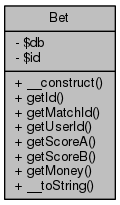
\includegraphics[scale=0.4]{UML_Bet.png}
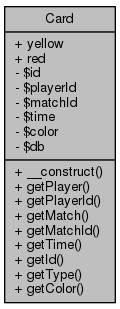
\includegraphics[scale=0.4]{UML_Card.png}
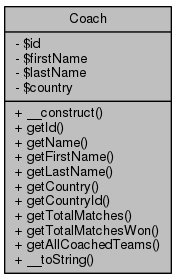
\includegraphics[scale=0.4]{UML_Coach.png}
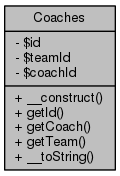
\includegraphics[scale=0.4]{UML_Coaches.png}
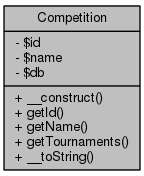
\includegraphics[scale=0.4]{UML_Competition.png}
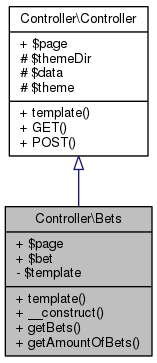
\includegraphics[scale=0.4]{UML_Controller_1_1Bets.png}
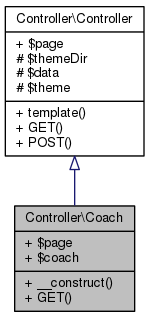
\includegraphics[scale=0.4]{UML_Controller_1_1Coach.png}
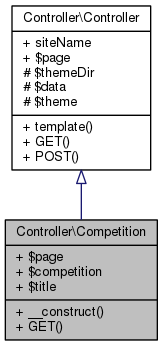
\includegraphics[scale=0.4]{UML_Controller_1_1Competition.png}
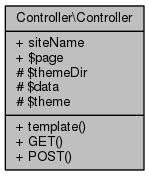
\includegraphics[scale=0.4]{UML_Controller_1_1Controller.png}
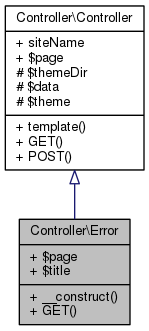
\includegraphics[scale=0.4]{UML_Controller_1_1Error.png}
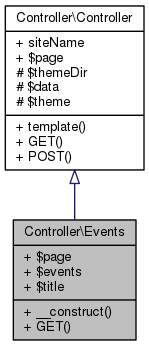
\includegraphics[scale=0.4]{UML_Controller_1_1Events.png}
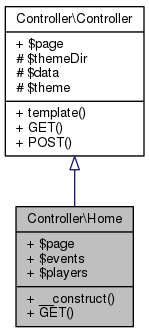
\includegraphics[scale=0.4]{UML_Controller_1_1Home.png}
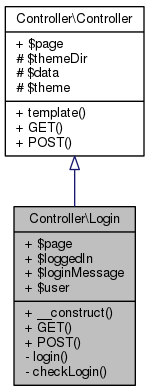
\includegraphics[scale=0.4]{UML_Controller_1_1Login.png}
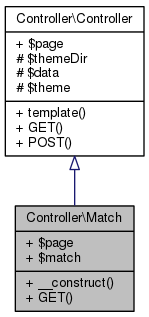
\includegraphics[scale=0.4]{UML_Controller_1_1Match.png}
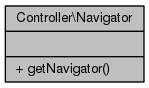
\includegraphics[scale=0.4]{UML_Controller_1_1Navigator.png}
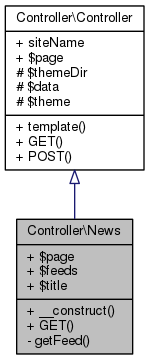
\includegraphics[scale=0.4]{UML_Controller_1_1News.png}
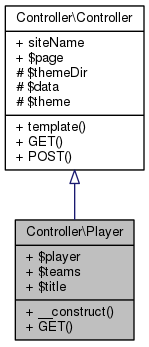
\includegraphics[scale=0.4]{UML_Controller_1_1Player.png}
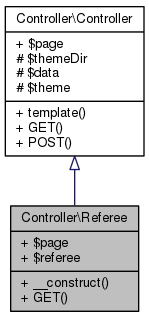
\includegraphics[scale=0.4]{UML_Controller_1_1Referee.png}
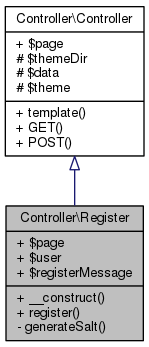
\includegraphics[scale=0.4]{UML_Controller_1_1Register.png}
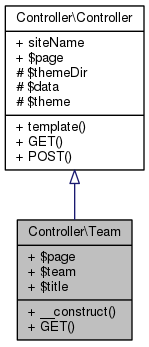
\includegraphics[scale=0.4]{UML_Controller_1_1Team.png}
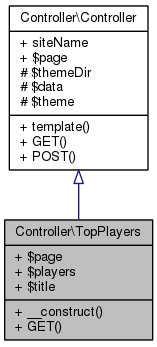
\includegraphics[scale=0.4]{UML_Controller_1_1TopPlayers.png}
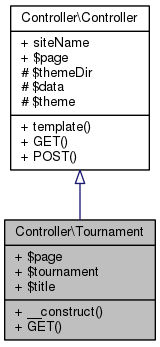
\includegraphics[scale=0.4]{UML_Controller_1_1Tournament.png}
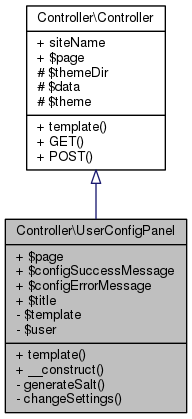
\includegraphics[scale=0.4]{UML_Controller_1_1UserConfigPanel.png}
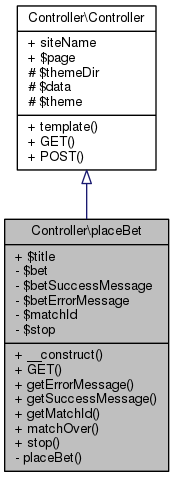
\includegraphics[scale=0.4]{UML_Controller_1_1placeBet.png}
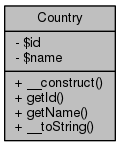
\includegraphics[scale=0.4]{UML_Country.png}
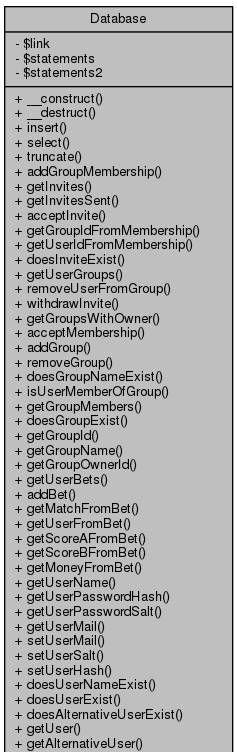
\includegraphics[scale=0.4]{UML_Database1.png}
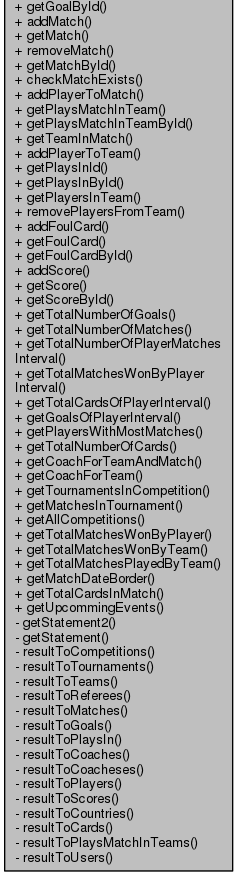
\includegraphics[scale=0.4]{UML_Database2.png}
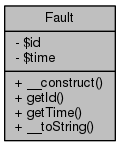
\includegraphics[scale=0.4]{UML_Fault.png}
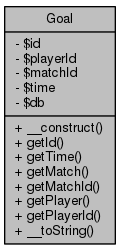
\includegraphics[scale=0.4]{UML_Goal.png}
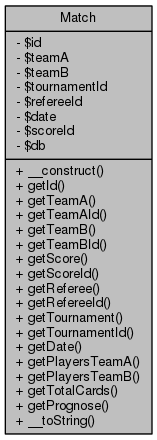
\includegraphics[scale=0.4]{UML_Match.png}
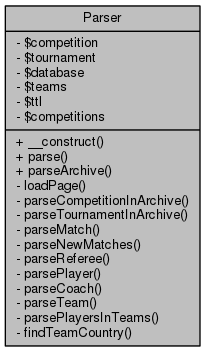
\includegraphics[scale=0.4]{UML_Parser.png}
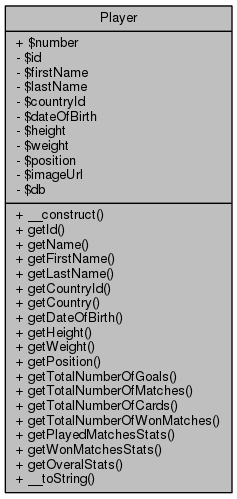
\includegraphics[scale=0.4]{UML_Player.png}
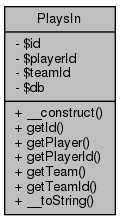
\includegraphics[scale=0.4]{UML_PlaysIn.png}
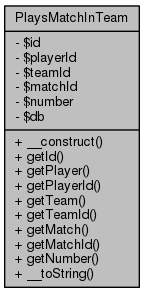
\includegraphics[scale=0.4]{UML_PlaysMatchInTeam.png}
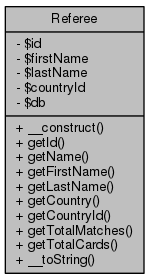
\includegraphics[scale=0.4]{UML_Referee.png}
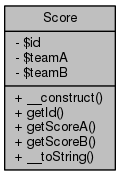
\includegraphics[scale=0.4]{UML_Score.png}
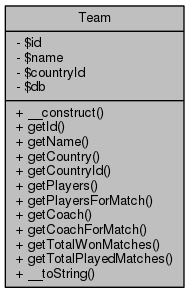
\includegraphics[scale=0.4]{UML_Team.png}
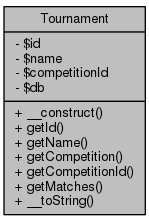
\includegraphics[scale=0.4]{UML_Tournament.png}
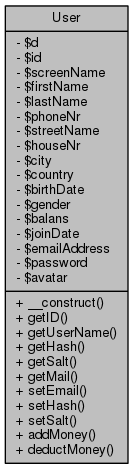
\includegraphics[scale=0.4]{UML_User.png}




\subsection{Parser}

De parser bestaat uit twee delen. De parseArchive functie zal, voor alle geselecteerde competities, alle wedstrijden van de afgelopen jaren gaan opzoeken en de data extraheren en in de database opslaan. Het is de bedoeling dat deze functie slechts eenmalig moet worden aangeroepen. Het andere deel, de crawler, zal regelmatig opnieuw worden uitgevoerd. Het zal de huidige competities in de gaten houden door nieuwe wedstrijden toe te voegen en de gegevens voor gespeelde wedstrijden te updaten.

Om het internetverkeer minder te belasten zal elke pagina die wordt binnengehaald gecached worden. Voor het archief zullen deze pagina's in de cache blijven, voor andere pagina's zal de pagina na een bepaalde tijd opnieuw worden gedownload.

De urls van de competities zijn hardcoded, maar vanaf deze pagina's worden alle matchen en teams door de parser ontdekt. Dus zelfs al zouden de urls wijzigen, dan zou dit haast geen werk kosten. Maar normaal moet de parser zonder problemen de komende jaren blijven werken.

Intern wordt gebruik gemaakt van de PHP Simple HTML DOM Parser om de pagina's om zo simpel de inhoud van een bepaalde tag op te kunnen vragen.

Uiteraard worden niet enkel de matchen geparset, maar zal de parser ook informatie over de spelers, teams, coaches en zelfs scheidsrechters zoeken en opslaan in de database.


\subsection{MVC}

% Mathias
Om geen spaghetti te maken van de implementatie van de pagina's, hebben we geopteerd voor het \emph{Model View Pattern}. We routeren onze urls via \emph{GluePHP} en \emph{mod\_rewrite}. Apache geeft alle urls door aan \emph{GluePHP}, welke a.h.v. gedefini\"eerde reguliere expressies de url zal mappen op een bepaalde klasse. Het framework zal dan de GET of POST functie (afhangende van het type request) uitvoeren op de nieuwe instantie van de juiste klasse. (In onze implementatie hebben we er echter voor gezorgd dat het framework dat object ook terugkeert, zodat we het verder kunnen gebruiken. Verder hebben we ook een catch-all controller toegevoegd aan het framework om error pagina's te kunnen genereren.)

Zo laten we \emph{GluePHP} een instantie van een \emph{Controller} aanmaken, die we bij het aanmaken de nodige datastructuren en informatie zal inladen. Op elke controller kunnen we dan een \emph{template} functie oproepen, die het overeenkomstige thema gedeelte zal insluiten op de pagina.


\begin{framed}
\begin{lstlisting}[language=php]
$urls = array(
	'error' => 'Controller\Error', //Catch all
	INSTALL_DIR . 'player/(\d+)' => 'Controller\Player',
	INSTALL_DIR . 'competition/(\d+)' => 'Controller\Competition',
	INSTALL_DIR . 'match/(\d+)' => 'Controller\Match',
	INSTALL_DIR . 'news' => 'Controller\News',
);

$controller = glue::stick($urls);
\end{lstlisting}
\end{framed}


\begin{framed}
\begin{lstlisting}[language=php]
//Include the header template
include(dirname(__FILE__) . '/theme/header.php');


//Include the theme part
$controller->template();


//Include the footer template
include(dirname(__FILE__) . '/theme/footer.php');
\end{lstlisting}
\end{framed}



\section{Database}

\subsection{Schema (ER-diagramma)}

Bij het aanvatten van een project zo omvangrijk in database structuur als dit, is het erg belangrijk om van in het begin een solide databasestructuur af te spreken.
Hiervoor hebben we dan ook meteen onze eerste samenkomst opge{\"e}ist.  We hebben goed nagedacht over welke zaken en hoe we deze met elkaar in verband gingen moeten brengen (wat niet zo eenvoudig was gezien niemand van onze groep een voetbalkenner is).

Het heeft alleszins zijn vruchten afgeworpen gezien onze huidige (ge{\"i}mplementeerde) databasestructuur erg weinig afwijkt van de eerste kribbel die we destijds op papier gezet hadden (met uitzondering van het nog niet ge{\"i}mplementeerde deel).

In de ERM zijn we vertrokken vanuit de entiteiten Match, Player en Team.  Hierop hebben we de rest van het 'voetbal' gedeelte van onze ERM gebouwd.  Ten slotte hebben we nog een 'gebruikers' gedeelte toegevoegd.

Gezien de omvang van de ERM kan het zijn dat u deze apart moet openen om deze voldoende leesbaar te kunnen bekijken.  (bijlages/ERM.png)


\begin{figure}[h!]
	\begin{center}
	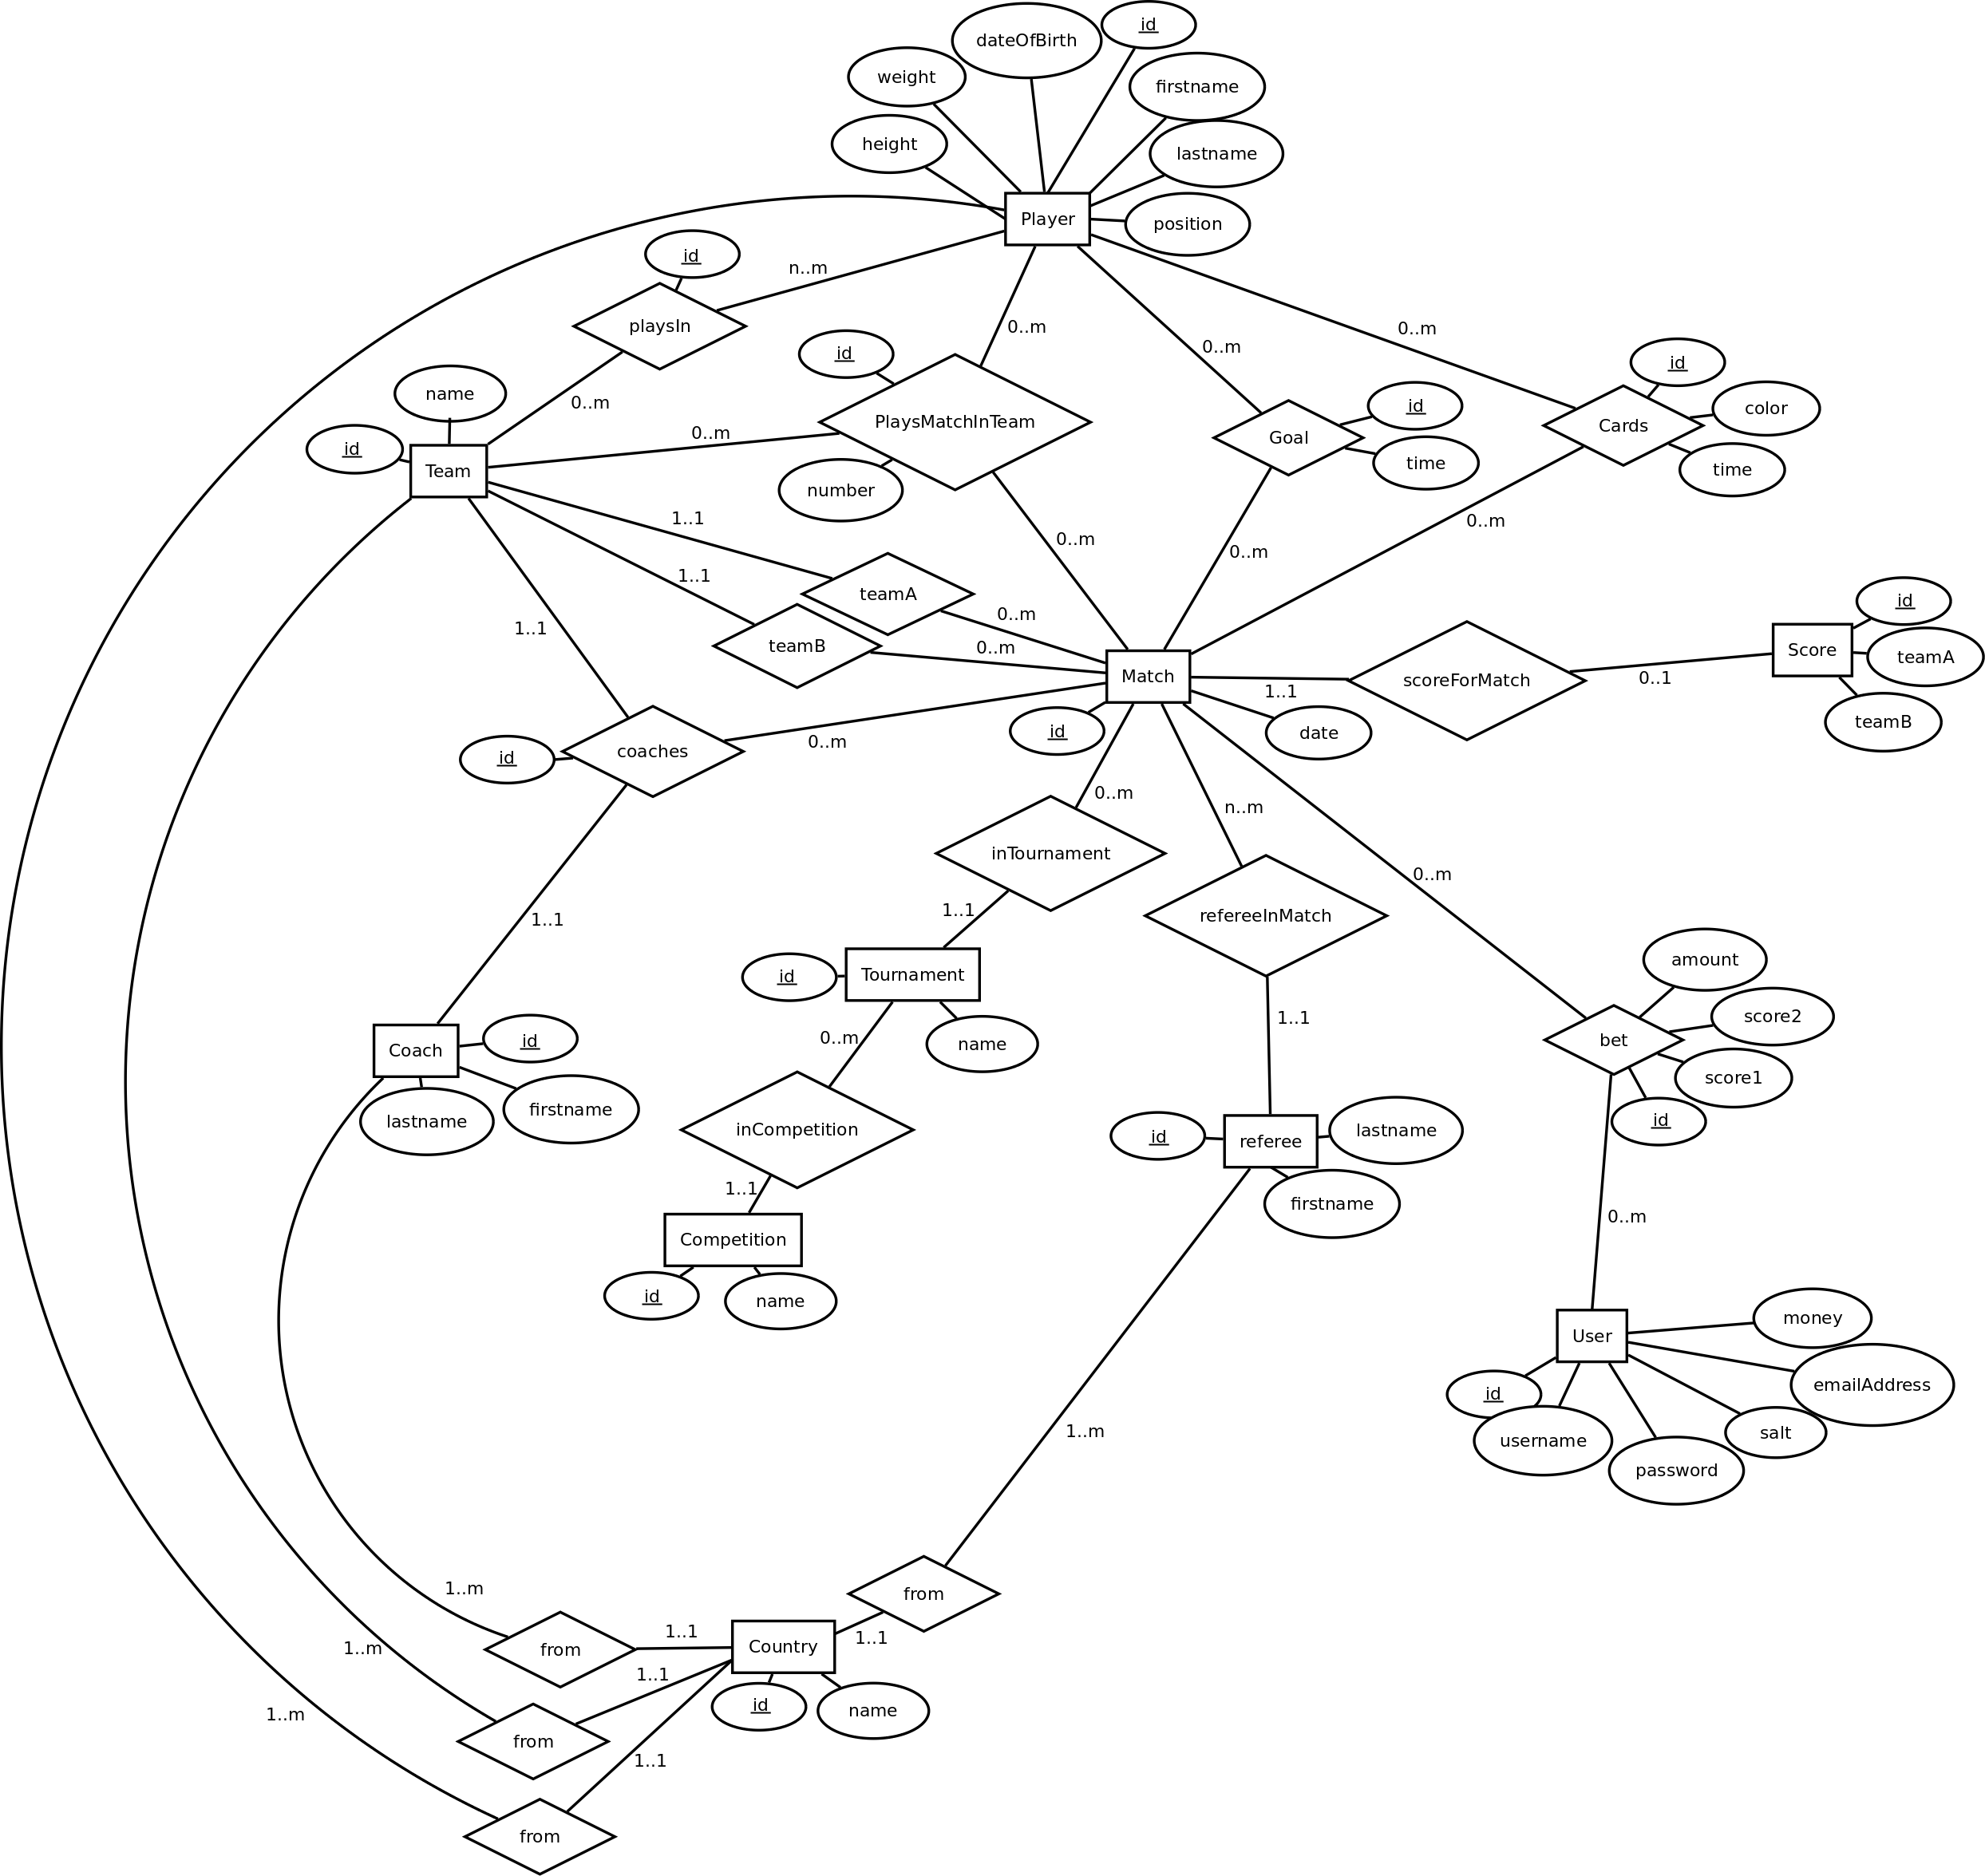
\includegraphics[scale=0.11]{ERM.png}

	\caption{ERM schema}
	\label{fig:speler}
	\end{center}
\end{figure}



\subsection{Constraints}

% Timo$




\section{User Interface}


De user interface concentreert zich vooral op matchen (met de voorspellingen en weddenschappen) en de spelers.
Gebruikers navigeren vanaf de homepage door de competities, seizoenen (binnen zo'n competitie) en krijgen dan een overzichtspagina van een bepaalde wedstrijd.
Op deze match pagina staat dan wat algemenen informatie zoals de score, scheidsrechters, ..., geflankeerd door de teams met hun spelers (voor die bepaalde match) opgelijst.

Gebruikers kunnen te allen tijde doorklikken op spelers, teams, coaches, competities, om zo telkens weer op een overzichtelijke pagina te komen waarop wat meer informatie staat.

Bij de spelers voorzien we de bezoeker van de nodige statistische data over een speler. Zo staan er het aantal gespeelde wedstrijden, gewonnen wedstrijden, kaarten en goals. Daarnaast staat er ook wat metadata over de spelers, zoals diens nationaliteit, positie op het veld, lengte, gewicht, etc.
Onderaan de pagina kan de bezoeker een grafiek zien met de wedstrijden van het laatste jaar. Daaronder staat een overzichts grafiek die de tijdlijn van de speler voorstelt. Met daarop alle matchen van zijn carri\`ere.

(Zie figuur \ref{fig:speler} p. \pageref{fig:speler} voor een voorbeeld van een speler pagina.)\\



Gebruikers kunnen op de website reeds registreren, inloggen, accountinstellingen wijzigen en bets plaatsen.
Het registratie,login en controle paneel is voorzien van voldoende checks die nagaan of de door de user opgegeven informatie correct is.  Zo kan een user bijvoorbeeld niet registreren met een syntactisch ongeldig emailadres of een gebruikersnaam die reeds bestaat.
\begin{figure}[h!]
	\begin{center}
	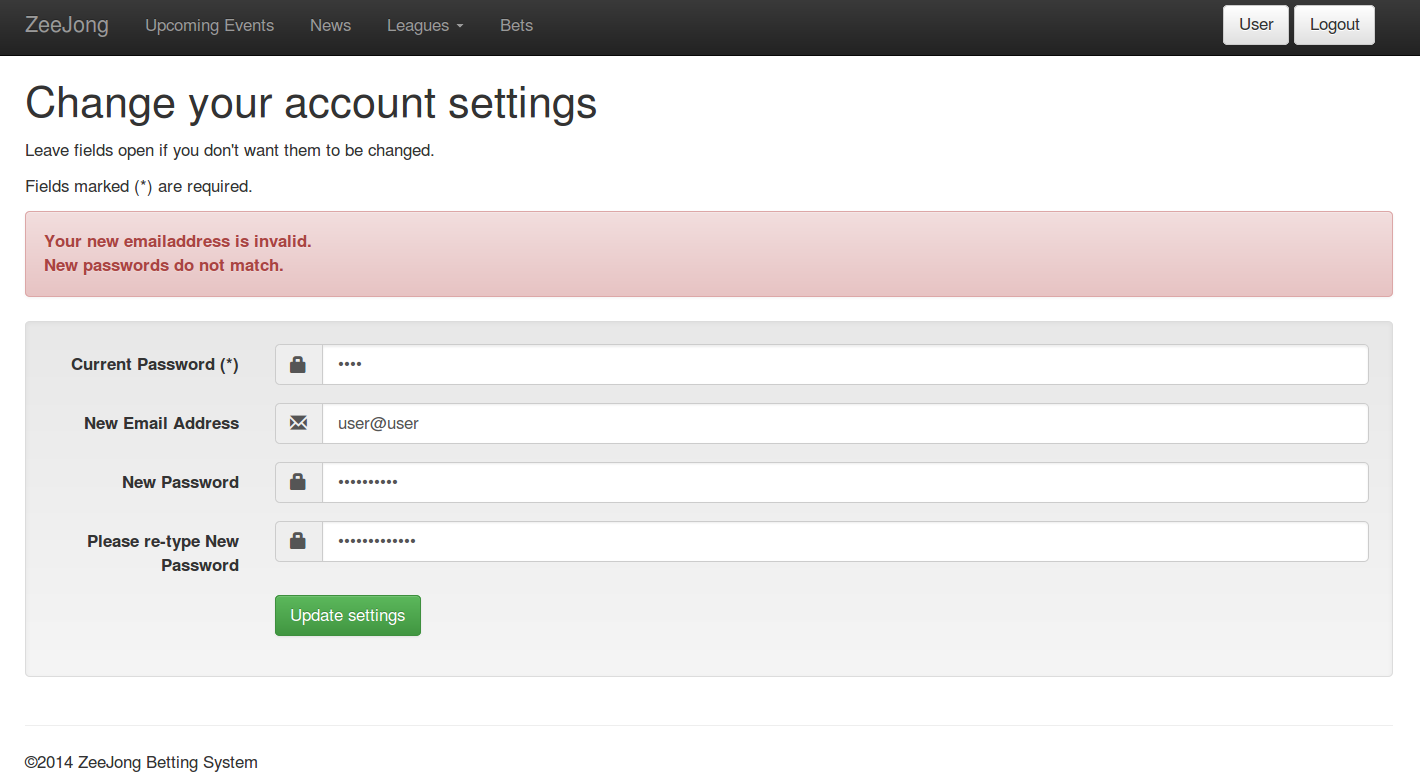
\includegraphics[scale=0.35]{changesettings.png}

	\caption{Schermafbeelding van het userConfigPanel}
	\label{fig:configPanel}
	\end{center}
\end{figure}
We hebben getracht ons user systeem volgens huidige maatstaven erg veilig te maken.
Wanneer een gebruiker registreert, dan wordt er een random salt gegenereerd en vervolgens wordt de sha256 hash berekend aan de hand van het gekozen wachtwoord, geconcateneerd met de salt.
In de database worden de salt en het gehashte wachtwoord opgeslagen.
Bij het inloggen wordt min of meer hetzelfde gedaan: de sha256 hash wordt wederom berekend aan de hand van de salt van de user (in de database) en het wachtwoord dat de user ingeeft.
Als de berekende hash dan overeenkomt met de hash van de user in de database, dan was het wachtwoord correct en is de gebruiker ingelogd.
\\\\
Een gebruiker kan reeds bets plaatsen op een score voor een bepaalde match en achteraf de reeds geplaatste bets bekijken.  Dit systeem is echter nog vrij primitief waardoor de bets bijvoorbeeld bij afloop van een match niet berekend worden en gewoon 'blijven staan'.
Het plaatsen van een bet gebeurt door naar de pagina van een bepaalde wedstrijd te gaan en op de 'bet' knop te drukken.  Vervolgens landt de gebruiker op een pagina bij welke hij een bepaalde score en geldbedrag kan kiezen.
\begin{figure}[h!]
	\begin{center}
	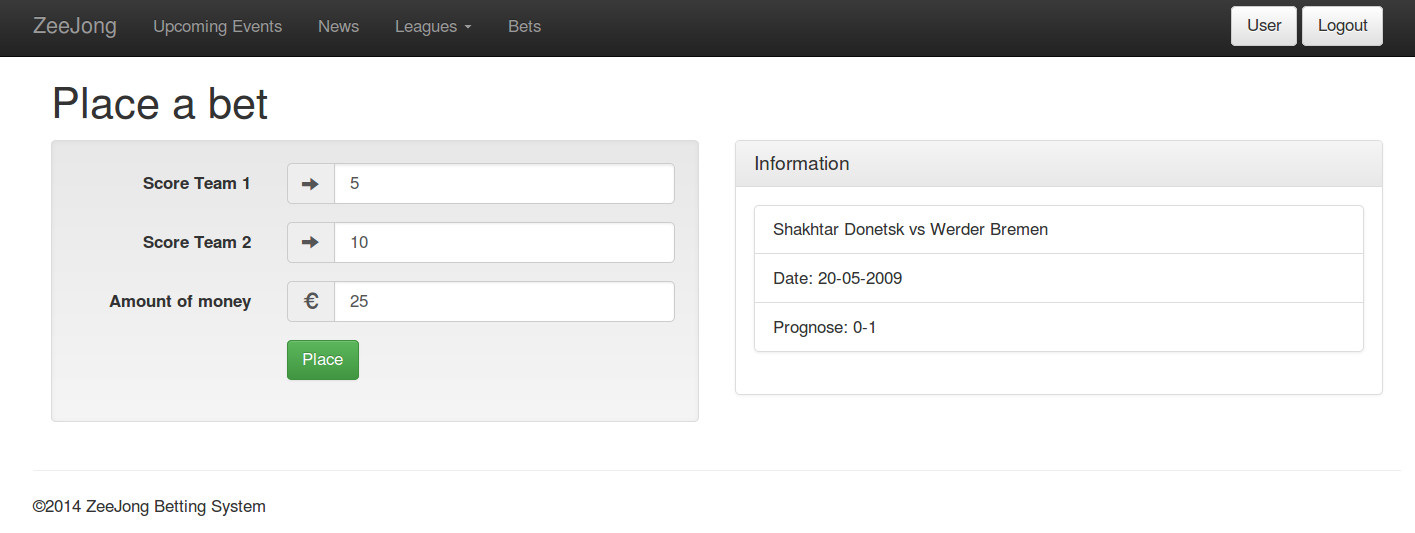
\includegraphics[scale=0.35]{placeBet.png}

	\caption{Schermafbeelding van de place bet pagina}
	\label{fig:placeBet}
	\end{center}
\end{figure}

\begin{figure}[h!]
	\begin{center}
	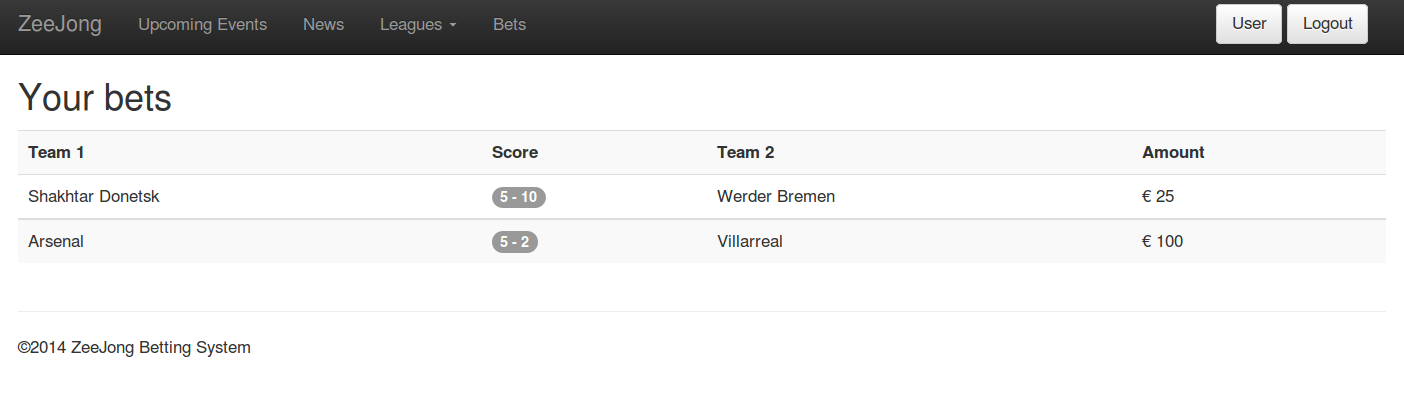
\includegraphics[scale=0.35]{bets.png}
	\caption{Schermafbeelding van de bets pagina}
	\label{fig:bets}
	\end{center}
\end{figure}






Om het design tot een goed einde te brengen hebben we gebruik gemaakt van het \emph{Bootstrap} 
framework. Hierdoor hadden we een stevige basis om op te steunen bij het stylen van de pagina's. (Voor de installatie pagina hebben we echter de minimalistische framework \emph{Pure CSS} gebruikt.)

De grafieken worden in javascript gerenderd op de html5 canvas d.m.v. de javascript module \emph{ChartJS}.

Intern hebben we slechts \'e\'en framework gebruikt, namelijk \emph{GluePHP}. Dit framework zet urls om in klasse objecten op basis van reguliere expressies. Zo konden we met Apache's \emph{mod\_rewrite} onze urls afhandelen.

\begin{figure}[h!]
	\begin{center}
	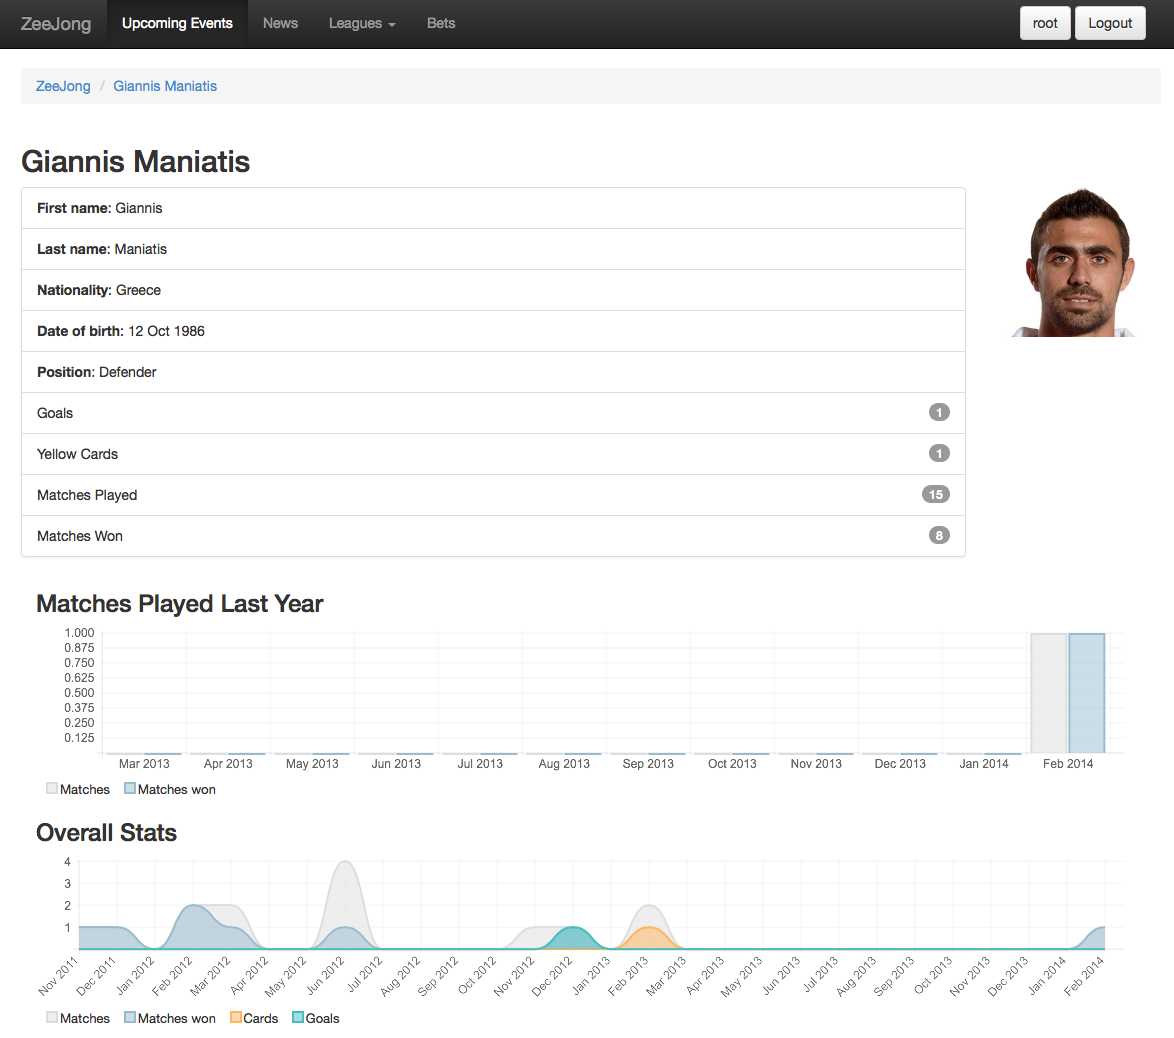
\includegraphics[scale=0.29]{player.png}

	\caption{Schermafbeelding van de speler pagina}
	\label{fig:speler}
	\end{center}
\end{figure}




\section{Extra Functionaliteit}


\subsection{Selector class}

%Timo
% gelieve dat de syntax in zo'n box te zetten



\paragraph{Selector}

Om te voorkomen dat er zeer veel verschillende queries geschreven moeten is er een wrapper geschreven die
deze queries automatisch genereert. Momenteel werkt deze wrapper alleen voor niet al te ingewikkelde select queries.

Bijvoorbeeld: We willen weten hoeveel goals een speler heeft gemaakt:
\begin{framed}
\begin{lstlisting}[language=php]
$sel = new Selector('Goal'); // Selecteer Goal column
$sel->filter([['playerId', '=', $playerId]]); // Filter op de speler
$sel->count(); // Tel het aantal resultaten.
\end{lstlisting}
\end{framed}


De selector kan dan aan de database worden gegeven die de sql query zal omzetten in een prepared statement en uitvoeren.
In dit geval zal de volgende query gegenereerd worden:
\begin{framed}
\begin{lstlisting}[language=php]
SELECT COUNT(*) FROM `Goal` WHERE (`playerId`=?)
\end{lstlisting}
\end{framed}

De gebruiker krijgt dan als resultaat een associatieve array terug met de values die geselecteerd zijn.\\

Hier nog enkele voorbeelden:

\paragraph{Voorbeeld 1}

Selecteer de spelers in een bepaald team
\begin{framed}
\begin{lstlisting}[language=php]
$sel = new Selector('PlaysIn');
$sel->filter([['teamId', '=', $teamId]]);
$sel->join('Player', 'playerId', 'id');
$sel->select('Player.*');
\end{lstlisting}
\end{framed}

\paragraph{Voorbeeld 2}

Tel hoeveel matchen een team gespeeld heeft
\begin{framed}
\begin{lstlisting}[language=php]
$sel = new Selector('Match');
$sel->filter(
    [
      // We moeten 1 van de teams zijn in deze match
      ['teamA', '=', $teamId],
      ['teamB' , '=', $teamId]
    ]);
// Als de scoreId niet NULL is hebben we gespeeld
$sel->filter([['scoreId', 'IS NOT NULL', '']]);
$sel->count();
\end{lstlisting}
\end{framed}









\subsection{Unit Test Framework}

Om ons ervan te vergewissen dat database de functie volledig werken, hebben we unit tests voorzien. Voor vele talen vind je dan zeer snel een zeer eenvoudig framework. Dit was echter niet meteen snel te vinden voor PHP. Daarom heeft Mathias zelf een test framework geschreven, waarmee het schrijven van unit tests veel gemakkelijk moet gaan.\\

Een test \emph{case} wordt gedeclareerd door simpelweg een PHP klasse te declareren. Een test \emph{section} binnen zulk een \emph{case} is dan gewoon een functie met daarin enkele uitvoerbare tests.
Voor het uitvoeren van de tests zijn er enkele \emph{REQUIRE} functies, zoals \emph{require\_true, require\_false, require\_equal, require\_notequal} en \emph{require\_exception}.

Een voorbeeld van een test bestand ziet er dan als volgt uit:

\begin{framed}
\begin{lstlisting}[language=php]
class Example extends UnitTest {
	
	public function AnotherTest() {
		
		$this->REQUIRE_EQUAL($var, $this->testVarA);
		$this->REQUIRE_NOTEQUAL('one', 'two');
		$this->REQUIRE_TRUE('one' == 'one');
		$this->REQUIRE_FALSE('one' == 'two');
		
	}
	
	public function ExceptionTest() {
		
		$this->BEGIN_REQUIRE_EXCEPTION();

		//A statement between BEGIN_REQUIRE and
		//END_REQUIRE should throw an exception
		//in order to make the performed test 'passed'.
		
		divide(2, 0);
		
		$this->END_REQUIRE_EXCEPTION();
		
	}	
	
}
\end{lstlisting}
\end{framed}


De gebruiker van het test framework plaatst alle te uitvoeren tests in de \emph{test} map, en het framework handelt de rest af. Je krijgt uiteraard een overzichtelijke html output bij het runnen van de tests (Zie figuur \ref{fig:unit-tests} p. \pageref{fig:unit-tests}).


\begin{figure}[h!]
	\begin{center}
	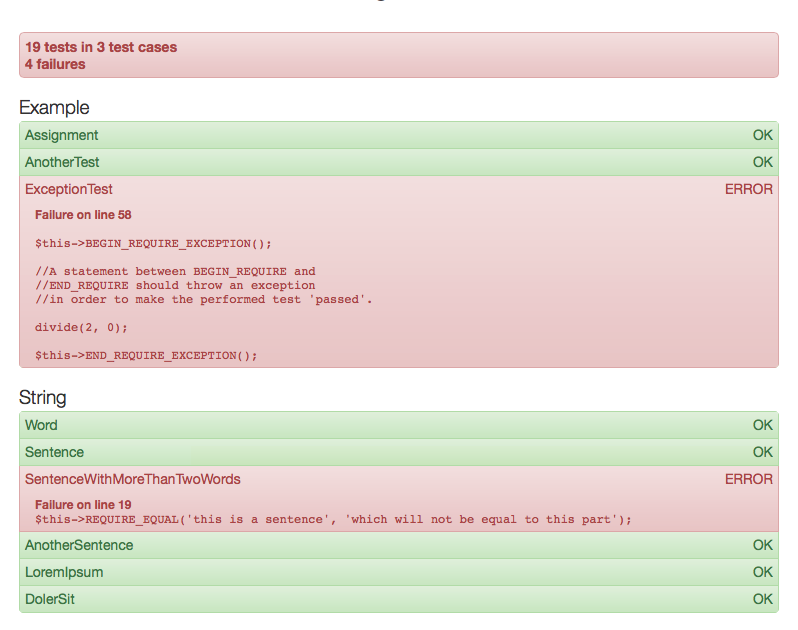
\includegraphics[scale=0.39]{unit-tests.png}

	\caption{HTML uitvoer van unit tests}
	\label{fig:unit-tests}
	\end{center}
\end{figure}




\subsection{RSS nieuwsfeed}

Om de gebruikers meer interessante inhoud op de website te bieden, hebben we onze site voorzien van een \emph{News} pagina, waarop we met RSS de laatste voetbal nieuwtjes binnehalen. Omdat zelf een RSS parser schrijven geen gemakkelijke klus is, gebruiken we \emph{SimplePie RSS}, een nieuwer alternatief voor \emph{Magpie RSS}.



\section{Planning}

Voor de volgende deadline verwachten we om het wedden op matchen volledig ge\"implementeerd te hebben. Daarnaast zou er ook een administratie pagina moeten komen voor dit geheel, waar de admins hun betting site in de gaten kunnen houden, en handmatig wedstrijden toevoegen of wijzigen.\\

Zoals we reeds deden, zullen we ook nu weer elke donderdag afspreken om afspraken te maken en issues te bespreken.



\section{Appendix}

\subsection{Volledige Queries}


\subsubsection{Tabellen}




    \paragraph{Bet}
        Bevat alle weddenschappen met de volgende informatie:
            match, score ploeg a, score ploeg b, tijdstip van weddenschap, de gebruiker,
            hoeveel geld er gewed is.
        De foreign keys zijn de gebruiker die de bet heeft gemaakt en de match waarop 
        de bet is gezet.
        
        \begin{framed}
        \begin{lstlisting}[language=sql]
CREATE TABLE IF NOT EXISTS `Bet` (
  `id` int(11) NOT NULL AUTO_INCREMENT,
  `matchId` int(11) NOT NULL,
  `score1` int(2) DEFAULT NULL,
  `score2` int(2) DEFAULT NULL,
  `time` int(3) NOT NULL,
  `userId` int(11) NOT NULL,
  `amount` int(11) NOT NULL,
  PRIMARY KEY (`id`),
  UNIQUE KEY `matchId_2` (`matchId`,`score1`,`score2`,`userId`),
  KEY `userId` (`userId`),
  KEY `matchId` (`matchId`)
) AUTO_INCREMENT=1 ;
        \end{lstlisting}
        \end{framed}

    \paragraph{Cards}
    
        Deze tabel bevat alle kaarten die spelers krijgen gedurende een wedstrijd.
        De tabel heeft dus als attributen de speler, match, kleur (geel/rood) en de tijd (d.i. het aantal verstreken minuten sinds het begin van de match)
    
        \begin{framed}
        \begin{lstlisting}[language=sql]
CREATE TABLE IF NOT EXISTS `Cards` (
  `id` int(11) NOT NULL AUTO_INCREMENT,
  `playerId` int(11) NOT NULL,
  `matchId` int(11) NOT NULL,
  `color` tinyint(1) NOT NULL,
  `time` int(3) NOT NULL,
  PRIMARY KEY (`id`),
  UNIQUE KEY `playerId_3` (`playerId`,`matchId`,`time`),
  KEY `playerId` (`playerId`,`matchId`),
  KEY `playerId_2` (`playerId`),
  KEY `matchId` (`matchId`)
) AUTO_INCREMENT=1 ;
        \end{lstlisting}
        \end{framed}
    
    
    \paragraph{Coach}
        Bevat alle coaches met de volgende informatie:
            naam, land
        Het land word gerefereerd door een foreign key.
        
        \begin{framed}
        \begin{lstlisting}[language=sql]
 CREATE TABLE IF NOT EXISTS `Coach` (
   `id` int(11) NOT NULL AUTO_INCREMENT,
   `firstname` varchar(50) NOT NULL,
   `lastname` varchar(50) NOT NULL,
   `country` int(11) NOT NULL,
   PRIMARY KEY (`id`),
   UNIQUE KEY `firstname` (`firstname`,`lastname`,`country`),
   KEY `country` (`country`),
   KEY `country_2` (`country`)
 ) AUTO_INCREMENT=1 ;
        \end{lstlisting}
        \end{framed}
        
        
        
    \paragraph{Coaches}
        Houdt bij wat de coach van een team is voor een bepaalde wedstrijd. Het bevat dus de volgende informatie:
            coach, team, match
        Coach, team en match zijn foreign keys.
        
        \begin{framed}
        \begin{lstlisting}[language=sql]
CREATE TABLE IF NOT EXISTS `Coaches` (
  `id` int(11) NOT NULL AUTO_INCREMENT,
  `coachId` int(11) NOT NULL,
  `teamId` int(11) NOT NULL,
  `matchId` int(11) NOT NULL,
  PRIMARY KEY (`id`),
  UNIQUE KEY `coachId_3` (`coachId`,`teamId`,`matchId`),
  KEY `coachId` (`coachId`,`teamId`),
  KEY `matchId` (`matchId`),
  KEY `teamId` (`teamId`),
  KEY `coachId_2` (`coachId`)
) AUTO_INCREMENT=1 ;
        \end{lstlisting}
        \end{framed}
        
        
        
    \paragraph{Competition}
        Bevat de namen van de competities.
        Bijvoorbeeld: World Cup, UEFA Europa League, ...
        
        \begin{framed}
        \begin{lstlisting}[language=sql]
CREATE TABLE IF NOT EXISTS `Competition` (
  `id` int(11) NOT NULL AUTO_INCREMENT,
  `name` varchar(50) NOT NULL,
  PRIMARY KEY (`id`),
  UNIQUE KEY `name` (`name`)
) AUTO_INCREMENT=1 ;
        \end{lstlisting}
        \end{framed}
        
        
        
        
    \paragraph{Country}
        Bevat de namen van landen.
        
        \begin{framed}
        \begin{lstlisting}[language=sql]
CREATE TABLE IF NOT EXISTS `Country` (
  `id` int(11) NOT NULL AUTO_INCREMENT,
  `name` varchar(50) NOT NULL,
  PRIMARY KEY (`id`),
  UNIQUE KEY `name` (`name`)
) AUTO_INCREMENT=1 ;
        \end{lstlisting}
        \end{framed}
        
        
        
        
    \paragraph{Goal}
        Bevat de volgende gegevens over een goal:
            speler, match, tijdstip
        De speler en de match zijn de foreign keys.
        
        \begin{framed}
        \begin{lstlisting}[language=sql]
CREATE TABLE IF NOT EXISTS `Goal` (
  `id` int(11) NOT NULL AUTO_INCREMENT,
  `playerId` int(11) NOT NULL,
  `matchId` int(11) NOT NULL,
  `time` int(3) NOT NULL,
  PRIMARY KEY (`id`),
  UNIQUE KEY `playerId_3` (`playerId`,`matchId`,`time`),
  KEY `playerId` (`playerId`,`matchId`),
  KEY `matchId` (`matchId`),
  KEY `playerId_2` (`playerId`)
) AUTO_INCREMENT=1 ;
        \end{lstlisting}
        \end{framed}
        
        
        
        
        
    \paragraph{Match}
        Bevat de volgende informatie over een match:
            de 2 teams, het tournament, de scheidsrechter, datum, de uitslag
        De teams, het tournament, de scheidsrechter en de uitslag zijn foreign keys.
        
        \begin{framed}
        \begin{lstlisting}[language=sql]
CREATE TABLE IF NOT EXISTS `Match` (
  `id` int(11) NOT NULL AUTO_INCREMENT,
  `teamA` int(11) NOT NULL,
  `teamB` int(11) NOT NULL,
  `tournamentId` int(11) NOT NULL,
  `refereeId` int(11) DEFAULT NULL,
  `date` int(11) NOT NULL,
  `scoreId` int(11) DEFAULT NULL,
  PRIMARY KEY (`id`),
  UNIQUE KEY `teamA_2` (`teamA`,`teamB`,`tournamentId`,`date`),
  KEY `teamA` (`teamA`,`teamB`),
  KEY `tournamentId` (`tournamentId`,`refereeId`),
  KEY `scoreId` (`scoreId`),
  KEY `refereeId` (`refereeId`),
  KEY `tournamentId_2` (`tournamentId`),
  KEY `teamB` (`teamB`)
) AUTO_INCREMENT=1 ;
        \end{lstlisting}
        \end{framed}
        
        
        
        
    \paragraph{Player}
        Bevat de volgende gegevens over een speler:
            naam, land, geboortedatum, lengte, gewicht, positie(aanvaller,verdediger,...)
        Het land is een foreign key.
        
        \begin{framed}
        \begin{lstlisting}[language=sql]
CREATE TABLE IF NOT EXISTS `Player` (
  `id` int(11) NOT NULL AUTO_INCREMENT,
  `firstname` varchar(50) NOT NULL,
  `lastname` varchar(50) NOT NULL,
  `country` int(11) NOT NULL,
  `dateOfBirth` int(11) DEFAULT NULL,
  `height` int(3) DEFAULT NULL,
  `weight` int(3) DEFAULT NULL,
  `position` varchar(50) DEFAULT NULL,
  PRIMARY KEY (`id`),
  UNIQUE KEY `firstname` (`firstname`,`lastname`,`country`,`dateOfBirth`),
  KEY `country` (`country`)
) AUTO_INCREMENT=1 ;
        \end{lstlisting}
        \end{framed}
        
        
        
        
    \paragraph{PlaysIn}
        Linkt de spelers met hun huidig team.
        De foreign keys zijn dus de speler en het team.
        Een speler heeft 1 huidig team, dit kan dus eventueel als extra informatie bij de speler worden opgeslagen.
        Hierdoor zal deze tabel overbodig worden.
        
        \begin{framed}
        \begin{lstlisting}[language=sql]
CREATE TABLE IF NOT EXISTS `PlaysIn` (
  `id` int(11) NOT NULL AUTO_INCREMENT,
  `playerId` int(11) NOT NULL,
  `teamId` int(11) NOT NULL,
  PRIMARY KEY (`id`),
  UNIQUE KEY `playerId_2` (`playerId`,`teamId`),
  KEY `playerId` (`playerId`),
  KEY `teamId` (`teamId`)
) AUTO_INCREMENT=1 ;
        \end{lstlisting}
        \end{framed}
        
        
        
    \paragraph{PlaysMatchInTeam}
        Houd bij welke spelers voor welk team speelden in een bepaalde match.
        De foreign keys zijn de speler, het team en de match.
        
        \begin{framed}
        \begin{lstlisting}[language=sql]
CREATE TABLE IF NOT EXISTS `PlaysMatchInTeam` (
  `id` int(11) NOT NULL AUTO_INCREMENT,
  `playerId` int(11) NOT NULL,
  `number` int(11) NOT NULL,
  `teamId` int(11) NOT NULL,
  `matchId` int(11) NOT NULL,
  PRIMARY KEY (`id`),
  UNIQUE KEY `playerId_2` (`playerId`,`teamId`,`matchId`),
  KEY `playerId` (`playerId`,`teamId`,`matchId`),
  KEY `teamId` (`teamId`),
  KEY `matchId` (`matchId`)
) AUTO_INCREMENT=1 ;
        \end{lstlisting}
        \end{framed}
        
        
        
    
    \paragraph{Referee}
        Bevat de volgende informatia over een scheidsrechter:
            naam, land
        Het land is een foreign key.
        
        \begin{framed}
        \begin{lstlisting}[language=sql]
CREATE TABLE IF NOT EXISTS `Referee` (
  `id` int(11) NOT NULL AUTO_INCREMENT,
  `firstname` varchar(50) NOT NULL,
  `lastname` varchar(50) NOT NULL,
  `countryId` int(11) NOT NULL,
  PRIMARY KEY (`id`),
  UNIQUE KEY `firstname` (`firstname`,`lastname`,`countryId`),
  KEY `countryId` (`countryId`)
) AUTO_INCREMENT=1 ;
        \end{lstlisting}
        \end{framed}
        
        
        
        
    \paragraph{Score}
        Bevat de uitslagen, de score van team 1 en van team 2.
        
        \begin{framed}
        \begin{lstlisting}[language=sql]
CREATE TABLE IF NOT EXISTS `Score` (
  `id` int(11) NOT NULL AUTO_INCREMENT,
  `teamA` int(11) DEFAULT NULL,
  `teamB` int(11) DEFAULT NULL,
  PRIMARY KEY (`id`),
  UNIQUE KEY `teamA` (`teamA`,`teamB`)
) AUTO_INCREMENT=1 ;
        \end{lstlisting}
        \end{framed}
        
        
        
    
    \paragraph{Team}
        Bevat de naam en het land van een team.
        Het land is de foreign key.
        
        \begin{framed}
        \begin{lstlisting}[language=sql]
CREATE TABLE IF NOT EXISTS `Team` (
  `id` int(11) NOT NULL AUTO_INCREMENT,
  `name` varchar(50) NOT NULL,
  `country` int(11) NOT NULL,
  PRIMARY KEY (`id`),
  UNIQUE KEY `name` (`name`,`country`),
  KEY `country` (`country`)
) AUTO_INCREMENT=1 ;
        \end{lstlisting}
        \end{framed}
        
        
        
        
    \paragraph{Tournament}
        Bevat de naam en bij welke competetie het hoort.
        De competitie is de foreign key.
        
        \begin{framed}
        \begin{lstlisting}[language=sql]
CREATE TABLE IF NOT EXISTS `Tournament` (
  `id` int(11) NOT NULL AUTO_INCREMENT,
  `name` varchar(50) NOT NULL,
  `competitionId` int(11) NOT NULL,
  PRIMARY KEY (`id`),
  UNIQUE KEY `name_2` (`name`,`competitionId`),
  KEY `competitionId` (`competitionId`),
  KEY `name` (`name`,`competitionId`)
) AUTO_INCREMENT=1 ;
        \end{lstlisting}
        \end{framed}
        
        
        
        
    \paragraph{User}
        Bevat informatie over de geregistreerde gebruikers(username, password, email, money).
        
        \begin{framed}
        \begin{lstlisting}[language=sql]
CREATE TABLE IF NOT EXISTS `User` (
  `id` int(11) NOT NULL AUTO_INCREMENT,
  `username` varchar(50) NOT NULL,
  `password` varchar(128) NOT NULL,
  `salt` varchar(128) NOT NULL,
  `emailAddress` varchar(50) NOT NULL,
  `money` int(11) DEFAULT '0',
  PRIMARY KEY (`id`),
  UNIQUE KEY `username` (`username`)
) AUTO_INCREMENT=1 ;
        \end{lstlisting}
        \end{framed}




\subsubsection{Constraints}

    \begin{framed}
    \begin{lstlisting}[language=sql]
--
-- Constraints for table `Bet`
--
ALTER TABLE `Bet`
  ADD CONSTRAINT `Bet_ibfk_2` FOREIGN KEY (`matchId`) REFERENCES `Match` (`id`),
  ADD CONSTRAINT `Bet_ibfk_1` FOREIGN KEY (`userId`) REFERENCES `User` (`id`);

--
-- Constraints for table `Cards`
--
ALTER TABLE `Cards`
  ADD CONSTRAINT `Cards_ibfk_2` FOREIGN KEY (`matchId`) REFERENCES `Match` (`id`),
  ADD CONSTRAINT `Cards_ibfk_1` FOREIGN KEY (`playerId`) REFERENCES `Player` (`id`);

--
-- Constraints for table `Coach`
--
ALTER TABLE `Coach`
  ADD CONSTRAINT `Coach_ibfk_1` FOREIGN KEY (`country`) REFERENCES `Country` (`id`);

--
-- Constraints for table `Coaches`
--
ALTER TABLE `Coaches`
  ADD CONSTRAINT `Coaches_ibfk_3` FOREIGN KEY (`matchId`) REFERENCES `Match` (`id`),
  ADD CONSTRAINT `Coaches_ibfk_1` FOREIGN KEY (`coachId`) REFERENCES `Coach` (`id`),
  ADD CONSTRAINT `Coaches_ibfk_2` FOREIGN KEY (`teamId`) REFERENCES `Team` (`id`);

--
-- Constraints for table `Goal`
--
ALTER TABLE `Goal`
  ADD CONSTRAINT `Goal_ibfk_2` FOREIGN KEY (`matchId`) REFERENCES `Match` (`id`),
  ADD CONSTRAINT `Goal_ibfk_1` FOREIGN KEY (`playerId`) REFERENCES `Player` (`id`);

--
-- Constraints for table `Match`
--
ALTER TABLE `Match`
  ADD CONSTRAINT `Match_ibfk_5` FOREIGN KEY (`scoreId`) REFERENCES `Score` (`id`),
  ADD CONSTRAINT `Match_ibfk_1` FOREIGN KEY (`teamA`) REFERENCES `Team` (`id`),
  ADD CONSTRAINT `Match_ibfk_2` FOREIGN KEY (`teamB`) REFERENCES `Team` (`id`),
  ADD CONSTRAINT `Match_ibfk_3` FOREIGN KEY (`tournamentId`) REFERENCES `Tournament` (`id`),
  ADD CONSTRAINT `Match_ibfk_4` FOREIGN KEY (`refereeId`) REFERENCES `Referee` (`id`);

--
-- Constraints for table `Player`
--
ALTER TABLE `Player`
  ADD CONSTRAINT `Player_ibfk_1` FOREIGN KEY (`country`) REFERENCES `Country` (`id`);

--
-- Constraints for table `PlaysIn`
--
ALTER TABLE `PlaysIn`
  ADD CONSTRAINT `PlaysIn_ibfk_2` FOREIGN KEY (`teamId`) REFERENCES `Team` (`id`),
  ADD CONSTRAINT `PlaysIn_ibfk_1` FOREIGN KEY (`playerId`) REFERENCES `Player` (`id`);

--
-- Constraints for table `PlaysMatchInTeam`
--
ALTER TABLE `PlaysMatchInTeam`
  ADD CONSTRAINT `PlaysMatchInTeam_ibfk_3` FOREIGN KEY (`matchId`) REFERENCES `Match` (`id`),
  ADD CONSTRAINT `PlaysMatchInTeam_ibfk_1` FOREIGN KEY (`playerId`) REFERENCES `Player` (`id`),
  ADD CONSTRAINT `PlaysMatchInTeam_ibfk_2` FOREIGN KEY (`teamId`) REFERENCES `Team` (`id`);

--
-- Constraints for table `Referee`
--
ALTER TABLE `Referee`
  ADD CONSTRAINT `Referee_ibfk_1` FOREIGN KEY (`countryId`) REFERENCES `Country` (`id`);

--
-- Constraints for table `Team`
--
ALTER TABLE `Team`
  ADD CONSTRAINT `Team_ibfk_1` FOREIGN KEY (`country`) REFERENCES `Country` (`id`);

--
-- Constraints for table `Tournament`
--
ALTER TABLE `Tournament`
  ADD CONSTRAINT `Tournament_ibfk_1` FOREIGN KEY (`competitionId`) REFERENCES `Competition` (`id`);
     \end{lstlisting}
     \end{framed}







%Elias
%Gelieve alle queries in de syntax highlighting 'veld' te zetten.

\subsubsection{Queries}


\paragraph{Getters: ID}

  Alle getters via id worden automatisch gegenereerd door een selector omdat deze allemaal een zeer gelijkaardige vorm hebben.
  Hier enkele voorbeelden, de id wordt telkens gegeven:

  \begin{framed}
  \begin{lstlisting}[language=sql]
  SELECT *
   FROM Country
   [WHERE id = ?];
  \end{lstlisting}
  \end{framed}

  \begin{framed}
  \begin{lstlisting}[language=sql]
  SELECT *
   FROM Match
   [WHERE id = ?];
  \end{lstlisting}
  \end{framed}

  \begin{framed}
  \begin{lstlisting}[language=sql]
  SELECT *
   FROM Player
   [WHERE id = ?];
  \end{lstlisting}
  \end{framed}


\paragraph{Getters: Attributen}

  Alle getters via attributen worden automatisch gegenereerd door een selector omdat deze allemaal een zeer gelijkaardige vorm hebben.
  Hier enkele voorbeelden, alle bepalende attributen, op de id na, worden telkens gegeven:

  \begin{framed}
  \begin{lstlisting}[language=sql]
  SELECT *
   FROM Country
   [WHERE name = ?];
  \end{lstlisting}
  \end{framed}

  \begin{framed}
  \begin{lstlisting}[language=sql]
  SELECT *
   FROM Match
   [WHERE teamA = ? AND
   teamB = ? AND
   date = ? AND
   tournamentId = ?];
  \end{lstlisting}
  \end{framed}

  \begin{framed}
  \begin{lstlisting}[language=sql]
  SELECT *
   FROM Player
   [WHERE firstname = ? AND
   lastname = ? AND
   country = ?];
  \end{lstlisting}
  \end{framed}




\emph{Naast de simpele get en insert queries, blijven er nog enkele ingewikkeldere queries over die we handmatig hebben geschreven.}


\paragraph{Gewonnen wedstrijden van speler binnen interval}

  Deze query vraagt de hoeveelheid matches waarbij de gegeven speler voor het winnende team speelde binnen een gegeven tijdspanne op.

  \begin{framed}
  \begin{lstlisting}[language=sql]
  SELECT COUNT(*)
   FROM `PlaysMatchInTeam`
   [JOIN `Match` ON `Match`.id = matchId]
   [JOIN `Score` ON `Score`.id = scoreId]
   [WHERE playerId = ? AND
   `Match`.date > ? AND
   `Match`.date < ? AND
      ((teamId = `Match`.teamA AND `Score`.teamA > `Score`.teamB) OR
      (teamID = `Match`.teamB AND `Score`.teamB > `Score`.teamA))];
  \end{lstlisting}
  \end{framed}


\paragraph{Gewonnen wedstrijden van speler}

  Deze query vraagt de hoeveelheid matches waarbij de gegeven speler in totaal voor het winnende team speelde.

  \begin{framed}
  \begin{lstlisting}[language=sql]
  SELECT COUNT(*)
   FROM `PlaysMatchInTeam`
   [JOIN `Match` ON `Match`.id = matchId]
   [JOIN `Score` ON `Score`.id = scoreId]
   [WHERE playerId = ? AND
      ((teamId = `Match`.teamA AND `Score`.teamA > `Score`.teamB) OR
      (teamID = `Match`.teamB AND `Score`.teamB > `Score`.teamA))];
  \end{lstlisting}
  \end{framed}




\paragraph{Gewonnen wedstrijden van team}

  Deze query vraagt de hoeveelheid matches die het gegeven team in totaal gewonnen heeft op.

  \begin{framed}
  \begin{lstlisting}[language=sql]
  SELECT COUNT(*)
   FROM `Team`
   [JOIN `Match` ON `Match`.teamA = `Team`.id OR `Match`.teamB = `Team`.id]
   [JOIN `Score` ON `Match`.scoreId = `Score`.id]
   [WHERE `Team`.id = ? AND
    ((`Match`.teamA = `Team`.id AND `Score`.teamA > `Score`.teamB) OR
    (`Match`.teamB = `Team`.id AND `Score`.teamB > `Score`.teamA)) ];

  \end{lstlisting}
  \end{framed}



\paragraph{Gespeelde wedstrijden}

  Deze query vraagt de hoeveelheid matches dat de gegeven speler in totaal gespeeld heeft op.

  \begin{framed}
  \begin{lstlisting}[language=sql]
  SELECT COUNT(*)
   FROM `PlaysMatchInTeam` AS p
   [INNER JOIN `Match` AS m ON p.matchIid = m.id]
   [WHERE p.playerId = ? AND
    m.date > ? AND
    m.date < ?];

  \end{lstlisting}
  \end{framed}



\paragraph{Kaarten binnen interval}

  Deze query vraagt de hoeveelheid strafkaarten dat de gegeven speler heeft gekregen binnen een bepaalde tijdspanne op.

  \begin{framed}
  \begin{lstlisting}[language=sql]
  SELECT COUNT(*)
   FROM `Cards`
   [JOIN `Match` ON `Match`.id = matchId]
   [WHERE playerId = ? AND
    `Match`.date > ? AND
    `Match`.date < ?];

  \end{lstlisting}
  \end{framed}



\paragraph{Goals binnen interval}

  Deze query vraagt de hoeveelheid goals dat de gegeven speler gescoord heeft binnen een bepaalde tijdspanne op.

  \begin{framed}
  \begin{lstlisting}[language=sql]
  SELECT COUNT(*)
   FROM `Goal`
   [JOIN `Match` ON `Match`.id = matchId]
   [WHERE playerId = ? AND
    `Match`.date > ? AND
    `Match`.date < ?];

  \end{lstlisting}
  \end{framed}


\paragraph{Meeste goals}

  Deze query vraagt een gegeven aantal spelers op met de meeste goals.

  \begin{framed}
  \begin{lstlisting}[language=sql]
  SELECT Player.*, COUNT(*) AS `playedMatches`
   FROM `Player`
   [JOIN `PlaysMatchInTeam` ON `PlaysMatchInTeam`.playerId = `Player.id`]
    [GROUP BY `Player`.id] 
    [ORDER BY `playedMatches` [DESC]]   
    LIMIT ?, ?;

  \end{lstlisting}
  \end{framed}





\subsection{Complexe UML}


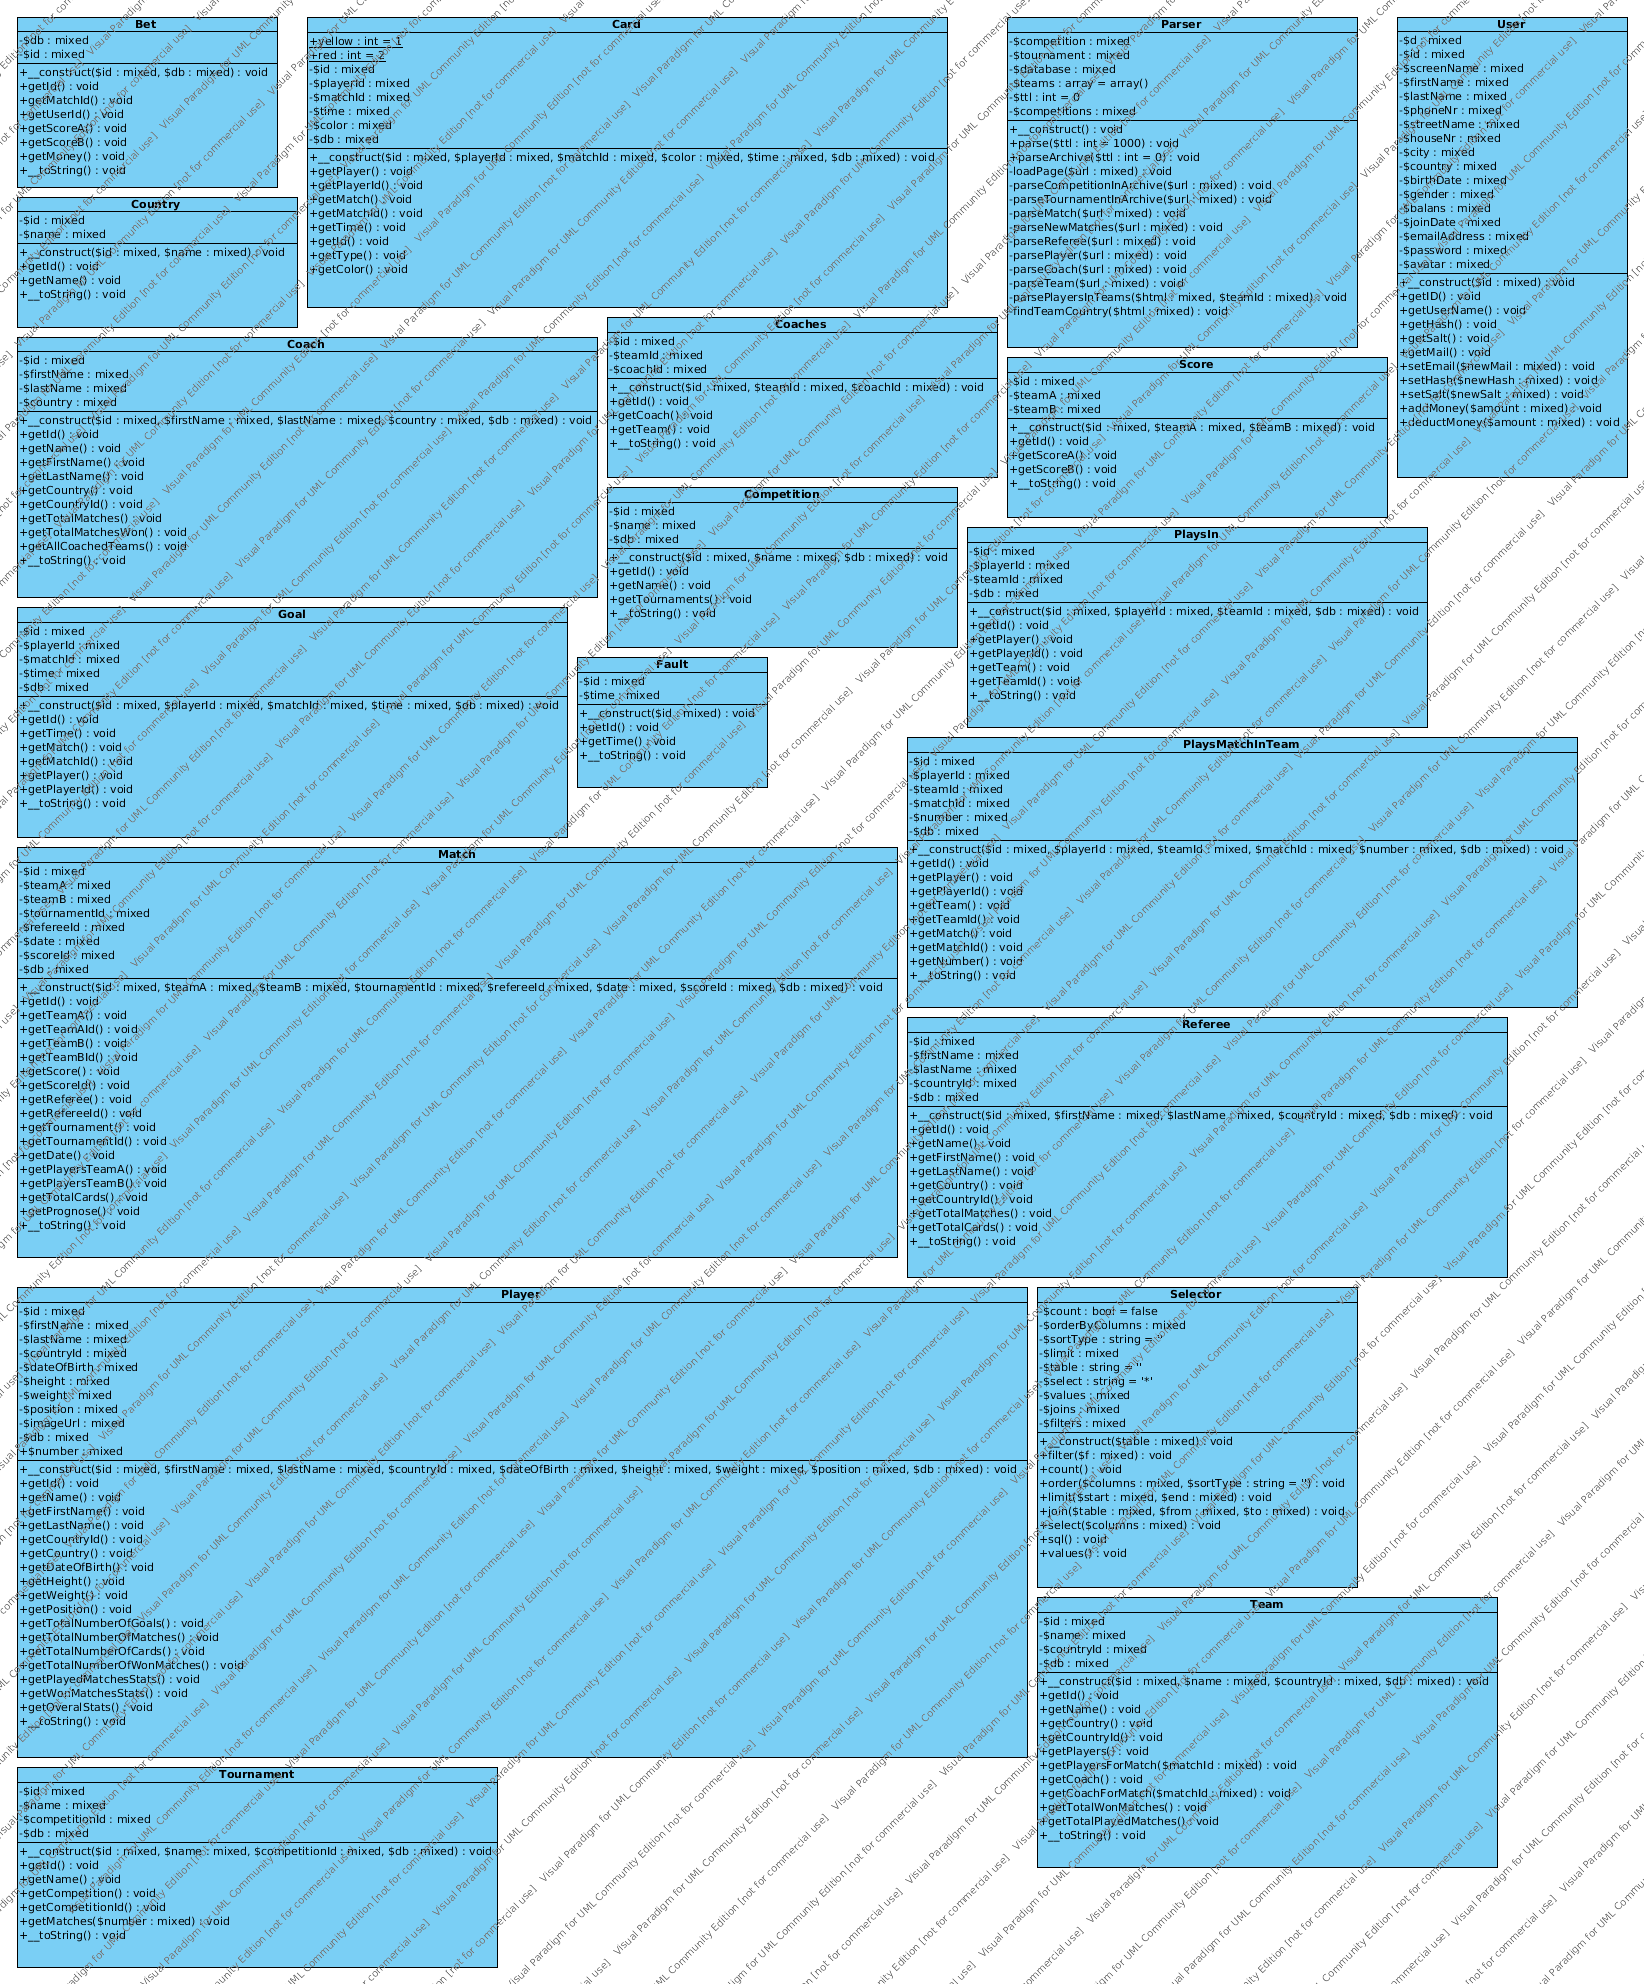
\includegraphics[scale=0.25]{UML_Classes.png}
\clearpage
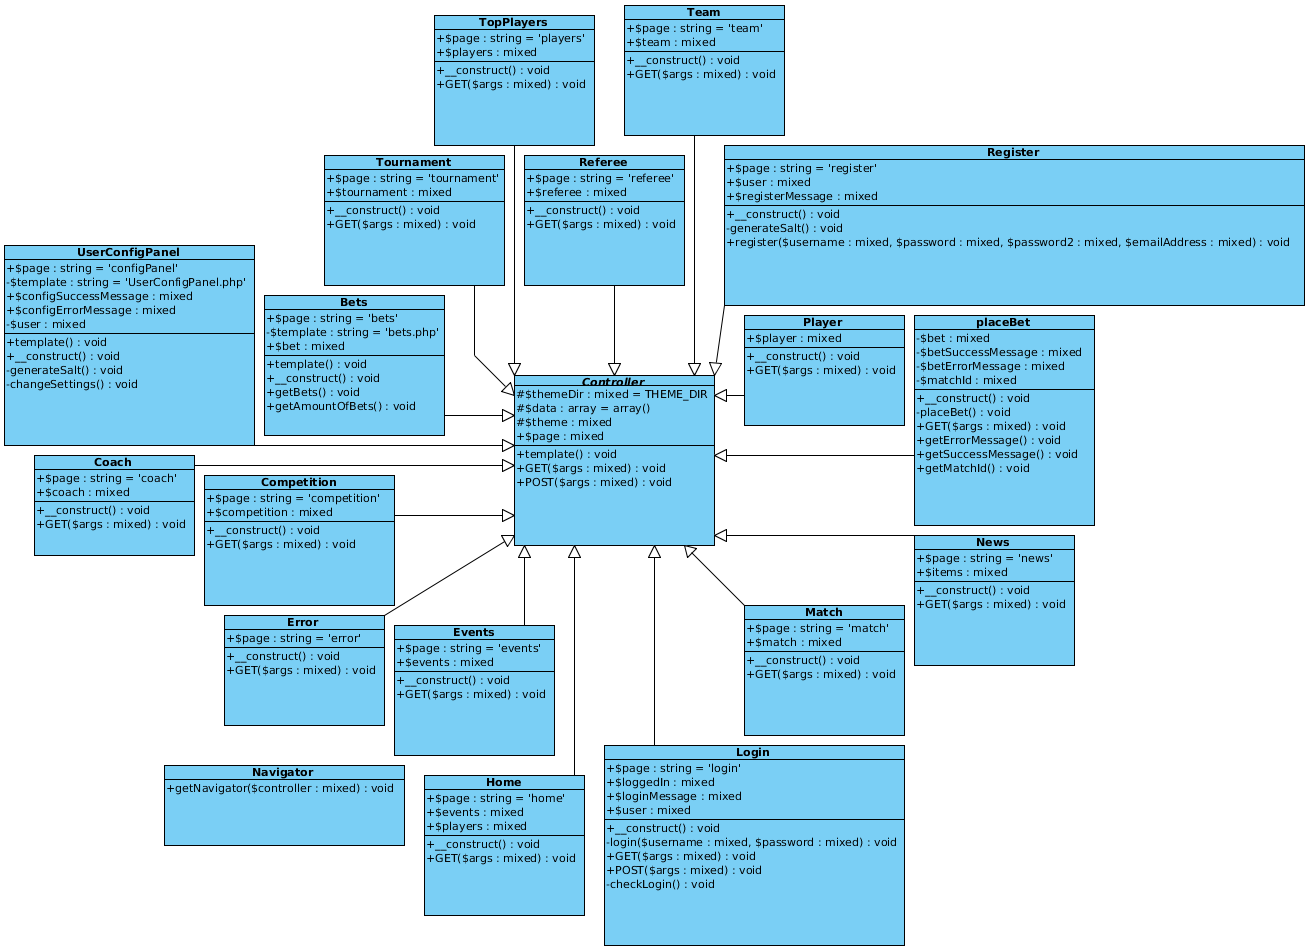
\includegraphics[scale=0.32]{UML_Controller.png}
\clearpage
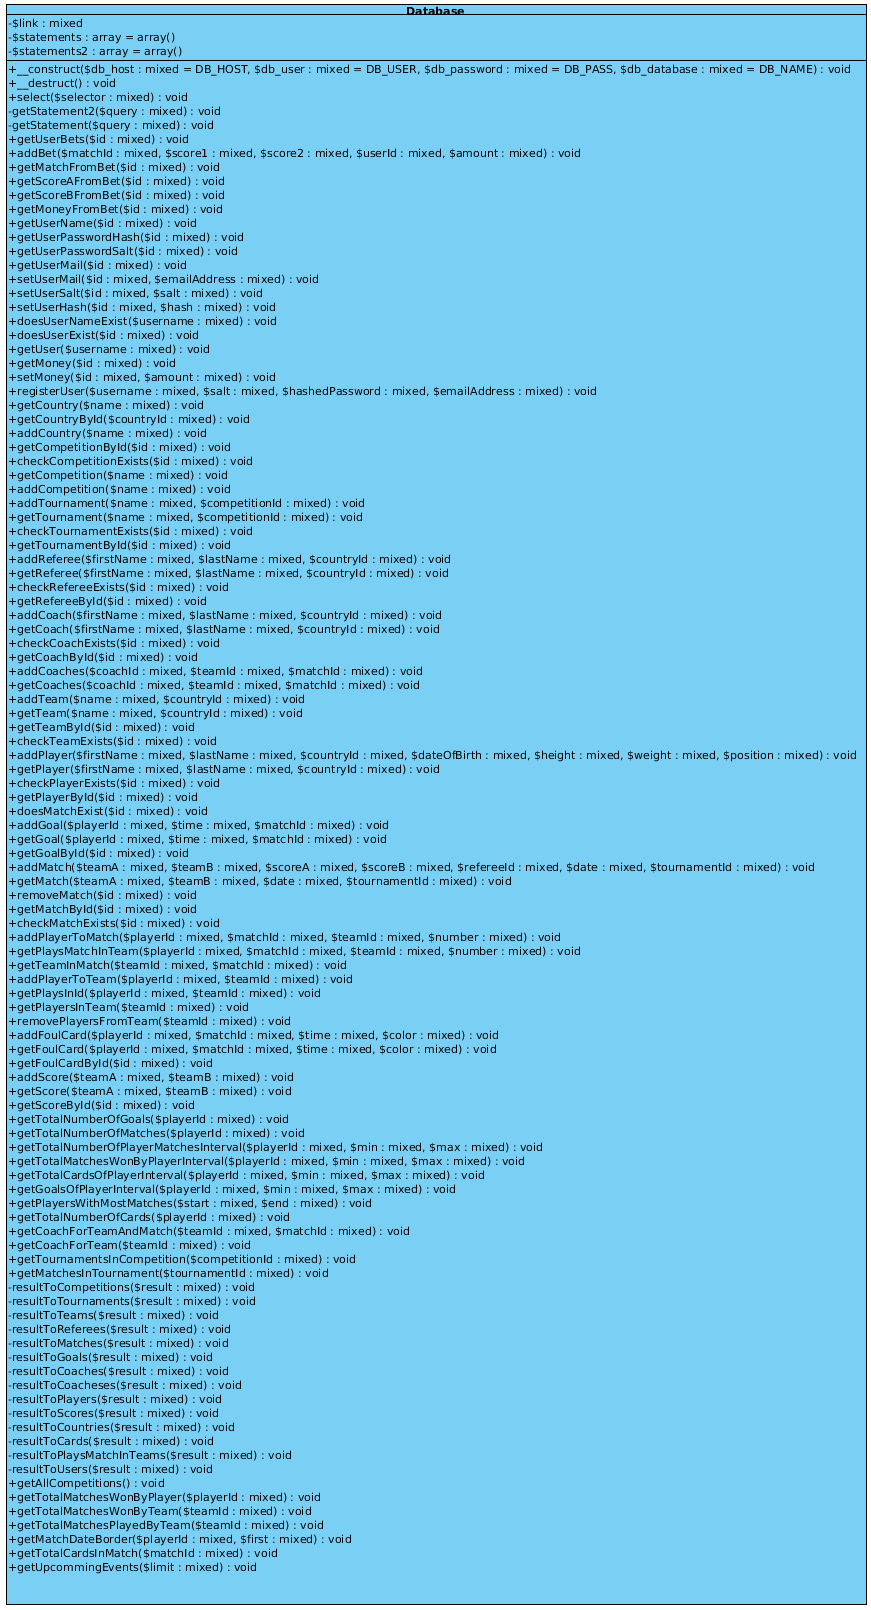
\includegraphics[scale=0.32]{UML_Database3.png}
\clearpage



\end{document}
